\chapter{Negotiation Skills}

Once one can present a venture, Joseph Hadzima remarks, one must then engage the people who want to know more. Mindy Garber takes over exactly there. In this MIT OpenCourseWare session, and in these companion notes curated by LazyingArt LLC, negotiation is treated not as executive polish or post hoc legal cleanup, but as part of the mechanics by which a young venture either holds together or comes apart. We will follow the lecture as it unfolds: first the stakes, then the split between adversarial and collaborative models, then the central move from positions to interests, and only after that the concrete startup cases in which the method is tested.

\section{Why Negotiation Belongs in a Startup Course}

Garber opens by fixing the stakes. Ventures often fail, she says, not because the technology collapses and not because the financing is absent, but because the people cannot keep working together. That fact gives the lecture its governing motivation. Negotiation is not ornamental business etiquette. It is part of the structure by which intellectual property, effort, and opportunity are either turned into a company or wasted.

Her self-positioning matters as well. She is both engineer and mediator. The engineer gathers the facts and seeks the optimal solution. The mediator helps people have a conversation they could not yet have, so that they can understand one another well enough to solve their own problem. The lecture never abandons the engineer's desire for structure, but it refuses the fantasy that a startup is only a technical system. A venture is a technical system inhabited by people whose motives, fears, and constraints are not self-revealing.

As editorial shorthand, and not as notation visible in the lecture, we may compress a negotiation into
\begin{equation}
N = (\mathcal{P}, \{I_p\}_{p\in\mathcal{P}}, O, R),
\end{equation}
where \(\mathcal{P}\) is the set of parties, \(I_p\) the interests of party \(p\), \(O\) the space of candidate options, and \(R\) the relationship and reputation constraints that survive the present exchange.

\begin{definition}
A negotiation is a structured attempt by a set of parties \(\mathcal{P}\) to move toward an outcome in \(O\), under the condition that each party carries interests \(I_p\) and that the relationship term \(R\) is usually not negligible.
\end{definition}

That last clause is already Garber's world. She does not begin with the legal instrument. She begins with the people who must continue speaking, deciding, revising, and working together.

\subsection{Question \& Answer}

\paragraph{Question.} Why is negotiation a venture skill rather than a legal afterthought?

\paragraph{Answer.} Because the venture is already negotiating before any formal legal event occurs. Cofounders negotiate motives, timing, sacrifice, roles, and ownership. Early employees negotiate culture and accountability. The company negotiates with customers, vendors, collaborators, and later with much larger organizations. If those conversations fail, the company may fail while the technology still works.

\section{Win-Lose, Collaboration, and Reputation}

From that opening Garber moves to the lecture's first conceptual split. There are many schools of negotiation, but at the level of first principles the lecture compresses them into two modes:
\begin{equation}
\mathrm{mode}(N) \in \{\text{win-lose},\ \text{collaborative problem solving}\}.
\end{equation}

In the win-lose model, one assumes a zero-sum game. If I gain, you lose. The relationship is peripheral. In the collaborative model, the two sides are working on a problem together. One still negotiates seriously, but one does so under the recognition that the relationship itself is part of the problem data.

Garber does not present this as mere ethical preference. The lecture's reasoning is structural. There is, she says, no such thing as one-and-done in startup life. The person across the table today may be the buyer, colleague, collaborator, or recommender tomorrow. Even if that exact individual moves to another company, the history does not vanish. In our shorthand, startup negotiation almost never lives in the degenerate regime
\[
R = \varnothing.
\]
More realistically,
\begin{equation}
R \neq \varnothing.
\end{equation}

This is why reputation appears so early in the lecture. ``Your reputation will precede you'' is not a moral slogan tacked onto bargaining theory. It is part of the constraint set. A startup that treats every meeting as a one-shot extraction game has misunderstood the environment in which it must survive.

\subsection{Question \& Answer}

\paragraph{Question.} Is negotiation fundamentally adversarial or collaborative?

\paragraph{Answer.} Garber's answer is that the adversarial temptation is always available, but the startup environment is structurally relational. Because the relationship persists, the faithful default is collaborative problem solving under constraint. The issue is not whether disagreement exists. The issue is whether we are willing to model the future consequences of how we handle it.

\section{Interests, Positions, and the Expansion of Options}

Only after the lecture has fixed the regime does it introduce its main analytic move. Garber asks what is, for the rest of the hour, the recurring question: what are your interests? She glosses these as needs, goals, hopes, and fears. The point is immediate. Many people cannot solve a problem because they have not yet identified what problem they are actually trying to solve.

\begin{definition}
A \emph{position} \(P_i\) is a stated demand, preferred term, or announced answer. An \emph{interest} \(I_i\) is the underlying need, constraint, aim, or fear that makes the position meaningful.
\end{definition}

The lecture's core chain may therefore be written as
\begin{equation}
P_i \longrightarrow I_i \longrightarrow O(I_i),
\end{equation}
where
\begin{equation}
O(I) = \{o : o \text{ satisfies the underlying interest } I\}.
\end{equation}

This is the chapter's central derivation. Once the interest beneath the position becomes visible, the option set widens.

\begin{proposition}
If a stated position \(P_i\) is only one means of satisfying an underlying interest \(I_i\), then exposing \(I_i\) enlarges the visible solution set:
\begin{equation}
\{P_i\} \subseteq O(I_i).
\end{equation}
\end{proposition}

\begin{proof}
Garber's fence example is enough. A party says, ``I want \(\$500\).'' That is the position. Asked why, the party answers that the fence was damaged and must be repaired. The interest is not intrinsically the money; it is the repair. Once that is visible, direct repair becomes a new admissible option. The single visible candidate has been replaced by a larger set.
\end{proof}

Garber's examples are deliberately concrete:
\begin{align}
P_{\text{fence}} &= \$500, &
I_{\text{fence}} &= \text{repair the fence},\\
o_1 &= \text{cash payment}, &
o_2 &= \text{direct repair by the other side}.
\end{align}

The same logic applies in technical argument. Engineers often arrive with what looks like the correct answer already fixed:
\begin{align}
P_{\text{code}} &= \text{use C++},\\
I_{\text{code}} &= \text{minimize time to an implementable system},\\
t_{\text{new language}} &\approx 6 \text{ months},\\
t_{\text{C++}} &\approx 3 \text{ weeks}.
\end{align}

The lecture's point is subtle. ``Use C++'' sounds technical and definitive, but even here it may only be a position. The interest is schedule. Once that becomes explicit, we can reason about time-to-implementation rather than treating the familiar language as sacred.

We may summarize Garber's procedure in the order she teaches it:
\begin{enumerate}
\item Start with the visible position \(P_i\).
\item Ask why that position is being defended.
\item Replace the declared answer by the underlying interest \(I_i\).
\item Search over \(O(I_i)\), not merely over variants of the original demand.
\item Compare options by how well they satisfy the interest.
\end{enumerate}

This is why Garber can later pause, during the Sandra case, and remind the class that even ``I want to raise capital'' may still only be a position. The interest lies one level deeper: what is the capital for, what does it protect, what does it enable, what risk does it answer?

\subsection{Question \& Answer}

\paragraph{Question.} What is the difference between a position and an interest?

\paragraph{Answer.} A position is the thing we say we want. An interest is the reason we want it. Garber's method is to keep asking why until the answer stops sounding like a bargaining move and starts sounding like a need, a fear, a constraint, or a goal. Only then do we see the actual option space.

\section{Founder Negotiation: First Questions and the Circle of Interests}

Having built the abstract mechanism, Garber narrows to startup life and, characteristically, makes the room work. The course is interactive. Students in the room and on Zoom are instructed to find partners and treat one another, for the moment, as cofounders. This matters. The lecture does not simply tell us the first questions; it makes the class feel what it is like to answer them under time pressure and social uncertainty.

Garber divides founder negotiation into three parts: first questions, founders agreements, and team agreements. She begins with the first questions. In compact form:
\begin{equation}
Q_0 = (\text{motivation},\ \text{success},\ \text{sacrifice}).
\end{equation}
In words: Why are you doing this? What does success look like? What are you giving up?

The third question has special force in the lecture. A founder may be giving up graduate school or a high-status job at Google. That sacrifice is not an ornament to the story. It tells us how the person is pricing the venture psychologically, which later shapes conflict around risk, speed, control, or exit.

Garber adds a second operation before any formal agreement enters. The partner must restate the answer. This is her active-listening move. The goal is not merely information transfer but evidence that both sides feel heard. Only after that does the lecture circle back to the central visual compression.

\begin{figure}[h]
\centering

\includegraphics[width=0.95\linewidth]{lecture_07_figure_02.png}
\caption{Circle-of-interests map for two founders.}
\end{figure}

This slide is the lecture's clearest diagram, and its geometry matters. The circle in the center is blank. The content lies outside it, in the lists attached by Garber's ``little sticks.'' One founder wants to be a successful entrepreneur, to learn what success requires, to make a difference, and to use technical skill in a startup. The other wants to solve an identified problem, learn about technology, challenge personal limits, and keep expanding detailed execution skills. The point is not to merge the lists into one slogan. The point is to place both sets of motives on one page at once.

\begin{figure}[h]
\centering
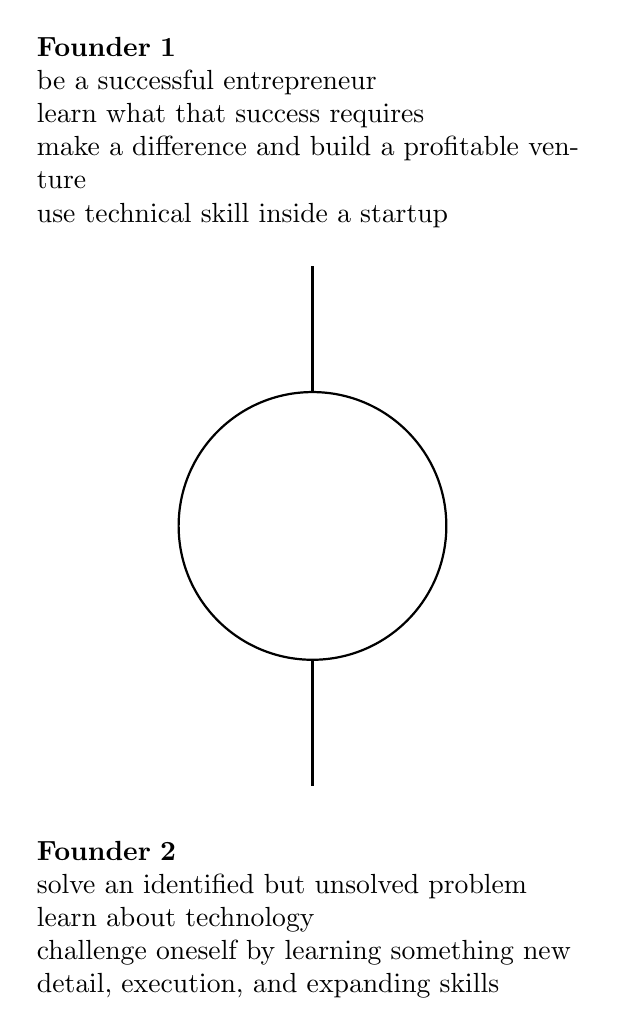
\begin{tikzpicture}[x=1cm,y=1cm]
\draw[thick] (0,0) circle (1.7);
\node[align=left,text width=7cm] at (0,5.0) {\textbf{Founder 1}\\
be a successful entrepreneur\\
learn what that success requires\\
make a difference and build a profitable venture\\
use technical skill inside a startup};
\draw[thick] (0,3.3) -- (0,1.7);
\node[align=left,text width=7cm] at (0,-5.0) {\textbf{Founder 2}\\
solve an identified but unsolved problem\\
learn about technology\\
challenge oneself by learning something new\\
detail, execution, and expanding skills};
\draw[thick] (0,-1.7) -- (0,-3.3);
\end{tikzpicture}
\caption{Editorial redraw of the circle-of-interests method in a taller, pocket-safe layout. The blank central circle is interpreted in the text as the shared discussion space \(C\).}
\end{figure}

As editorial shorthand we may therefore write
\begin{equation}
I_{\mathrm{F1}},\ I_{\mathrm{F2}} \longrightarrow C,
\end{equation}
where \(C\) is the shared page or conversational space, not yet the company itself. The blankness of the center is part of the point. Before we decide terms, we make the motives visible.

\begin{definition}
A \emph{circle of interests} is a one-page map that places several parties' interests around a shared discussion space so that hidden motives can be discussed before they harden into conflict.
\end{definition}

Garber's example is revealing because the founders had a good idea and both wanted to pursue it, yet they had not actually discussed why each wanted to do so. The diagram does not decorate the negotiation. It prevents the parties from negotiating blind.

\subsection{Question \& Answer}

\paragraph{Question.} How do we make hidden founder motives visible before conflict arrives?

\paragraph{Answer.} Garber's answer is procedural. Ask the first questions, restate the answers so that each side feels heard, and then write the resulting interests onto a common page. The circle does not solve the disagreement by itself; it creates the conditions under which the disagreement can be understood.

\section{From Founder Fit to Formal Agreements}

From the first questions, the lecture broadens to the thicker internal constitution of the company. This part of the hour is cumulative rather than theorem-like. Garber moves from honest assessment of cofounder fit, to founders agreements, to team agreements, and finally to the deadlock question that any equal founding pair must eventually face.

The honest-assessment portion is easily oversimplified if we read too fast. Garber is not saying that founders must begin with perfectly complementary technical backgrounds. Two mechanical engineers may found a company together. What matters is that they understand which skills are present, which are absent, and how the missing capabilities will later enter the firm.

The founders agreement then formalizes the obvious questions that people prefer to postpone: who owns what, who is contributing what, how equity will be discussed, and what happens if one founder leaves. Garber is especially insistent about this last point. One cannot safely defer the question of what occurs if the inventor departs, or if a founder who once did all the work later does less as the company grows. The lecture frames this not as moral complaint but as valuation: what are the pieces, who is contributing them, and how should those contributions be discussed honestly?

The team agreement moves from ownership to operating practice. Garber treats it as the startup's internal constitution. It covers, among other things,
\begin{itemize}
\item the culture the founders want to inhabit,
\item norms of behavior and communication,
\item meeting cadence and tools,
\item roles and accountability,
\item the procedure by which decisions are made,
\item the language by which the team can later revisit what it once agreed.
\end{itemize}

That last item is central to Garber's view. An agreement is valuable not only because it fixes a rule, but because it gives the team neutral language for repair. We do not have to begin from accusation; we can begin from what we previously said we would do, and then ask whether it still works.

This is also where the lecture's cultural point belongs. If the founders do not define culture, the first employees will define it for them. Garber puts the matter almost constitutionally: the startup has a rare chance to decide how people will work together before habits harden.

Only after all of this does the lecture arrive at the formal deadlock question. Many cofounders begin in structural symmetry:
\begin{equation}
s_1 = s_2 = 0.5.
\end{equation}

Garber does not reject the arrangement; she notes that it is extremely common. But she does insist that it creates a structural risk, so the team must have tools for disagreement. The classroom suggestions fall into several families: honest discussion, stepping back, consulting a neutral adviser, mediation, and distinguishing decisions that can be reversed from those that cannot. Editorially we may compress that distinction into
\begin{equation}
D \in \{D_{\text{one-way}},\ D_{\text{two-way}}\}.
\end{equation}
A one-way decision is difficult to reverse and therefore requires slower resolution. A two-way decision can be tested and revisited.

Garber's lawyer anecdote then appears as a foil rather than a conclusion:
\begin{equation}
(s_1,s_2) = (0.51,0.49).
\end{equation}

\begin{remark}
The lecture does not endorse \(0.51/0.49\) as a theorem of startup design. It appears as a litigation-minded lawyer's response to deadlock. Garber's own aim is to give founders better tools than litigation.
\end{remark}

Her actual advice is much closer to a decision rule:
\begin{equation}
D_{\text{two-way}} \Rightarrow \text{test, observe, revisit}, \qquad
D_{\text{one-way}} \Rightarrow \text{slow down, deliberate, and if needed seek help}.
\end{equation}

She even adds the temporal dimension: revisit these agreements periodically. Her own practice is to conduct cofounder check-ins every several months, not to ask only what the company is doing, but how the people are working together.

\subsection{Question \& Answer}

\paragraph{Question.} What should equal cofounders do when they disagree?

\paragraph{Answer.} They should not reach first for a magical decider. Garber's sequence is more disciplined: surface the disagreement honestly, decide whether the decision is reversible, bring in neutral advice if needed, and make sure the company has already defined what its escalation path will be. Equality is workable, but only if the founders treat disagreement as a design problem rather than as a personal surprise.

\section{The Sandra Case: A Negotiation Failure in Slow Motion}

At this point the lecture slows down and becomes case-based. Garber introduces the Sandra example as a true MIT story, and she does so in a deliberately staged way: first the overview, then the separate interests, then possible agreements, and only then the reveal.

\begin{figure}[h]
\centering

\includegraphics[width=0.95\linewidth]{lecture_07_figure_03.png}
\caption{Overview of the Sandra-undergraduates negotiation case.}
\end{figure}

The slide gives the ordered structure. Sandra has a prototype, but it can process only one cup of crude oil at a time. Several undergraduates hear about the invention, meet Sandra, and move toward the \(100\text{K}\) competition and perhaps a company. The relationship between the inventor and the undergraduates is never documented. The students then invest heavily in the business plan and in connections with major oil-processing executives. Just before the competition, Sandra considers pulling out on the ground that the invention is not ready.

In compact form:
\begin{align}
q_{\text{prototype}} &= 1 \text{ cup at a time},\\
A_{\text{written}} &= \varnothing,\\
\text{student investment} &= \text{already substantial},\\
\text{withdrawal point} &= \text{just before the competition}.
\end{align}

Garber then asks the class to do what the lecture has been building toward: identify the interests. The students may want experience, excitement, career direction, access to senior executives, resume value, or even a future job if the venture succeeds. Sandra wants to protect her intellectual property, keep control over what happens to her invention, avoid reputational harm in her field, and avoid presenting a technology as ready when scaling from one cup to industrial throughput is still unresolved.

This is where Garber carefully warns the room that inferred interests are not guaranteed to be correct. In mediation, she says, one can suggest an interest and be told immediately that it is wrong. Still, without trying to surface the interests, one has no serious way to search for agreement.

The class then generates agreements. The lecture does not collapse this into a single preferred answer, which is part of its power. Instead it shows the option space opening once the interests are named:
\begin{itemize}
\item Sandra could license the invention to a joint venture while remaining an advisor rather than a cofounder.
\item Equity could be tied to the set of functions required for the company rather than to one undifferentiated notion of contribution.
\item The IP could be protected while operational control is distributed.
\item Instead of forcing an immediate startup, the parties could move first into a research-and-grants phase devoted to scaling and validation.
\end{itemize}

At exactly this point Garber pauses to refine the earlier mathematics. Even ``I want to raise capital,'' she says, may still be only a position. We must still ask what the capital is meant to do. The Sandra case therefore doubles as a second pass through the position-interest distinction.

Then comes the reveal: there was no agreement. More importantly, there was no real conversation about what the students wanted and what Sandra wanted. Garber had even offered to help as a neutral third party, but the students assumed the effort itself would somehow resolve the underlying structure. It did not. Sandra eventually took the invention and formed a company with a different group of people.

\subsection{Question \& Answer}

\paragraph{Question.} Why did effort, enthusiasm, and opportunity still fail to produce an agreement?

\paragraph{Answer.} Because none of those things substitutes for negotiation. The students had labor and optimism; Sandra had control of the invention. But the parties never stabilized the relationship, never documented it, and never tested whether their preferred future was even the same future. The case is a failure not of energy but of explicit conversation.

\section{Negotiation Within and Beyond the Company}

After the Sandra case, Garber widens the scope again. The same method survives, but the environment becomes more complicated. Once we move inside a company, negotiations may no longer be simple two-party exchanges; power becomes asymmetric, legal issues become live, and confidentiality becomes tighter.

\begin{figure}[h]
\centering

\includegraphics[width=0.95\linewidth]{lecture_07_figure_04.png}
\caption{Internal-company negotiation complications.}
\end{figure}

The slide gives a clean checklist: there may be more than two parties, differences in ``power levels,'' legal ramifications, and a further level of confidentiality. Editorially we may write
\begin{equation}
n > 2
\end{equation}
and
\begin{equation}
N_{\text{internal}} = (\mathcal{P}, \{I_p\}_{p\in\mathcal{P}}, O, R, L, K),
\end{equation}
where \(L\) records legal implications and \(K\) records confidentiality constraints.

Garber immediately adds the lecture's recurring refrain: even here she still draws her little circle of interests. In other words, the model does not change; the complication set grows.

\paragraph{The Judy case.} The first application is internal. Judy wants a promotion to marketing manager. Garber's method is stakeholder decomposition:
\begin{equation}
S_{\text{Judy}} = \{\text{Judy},\ \text{manager},\ \text{company},\ \text{teammates}\}.
\end{equation}
Judy wants challenge, recognition, greater responsibility, supervisory opportunity, and a chance to use newly acquired skills. Her manager wants to appear capable of developing employees but also needs the existing work completed. The company wants revenue, effective leadership, employee growth, diversity, and successful projects. Teammates may want promotion opportunities of their own.

Garber then helps Judy move from diffuse aspiration to structured preparation. Judy receives a list of marketing functions, puts them into a spreadsheet, and assigns weights:
\begin{equation}
w_j \in \{1,2,3\}, \qquad \text{with larger } w_j \text{ indicating greater importance.}
\end{equation}
The spreadsheet is not the theorem; it is the mechanism by which a vague ambition becomes an ordered plan. Judy then walks into the conversation not merely saying, ``Promote me,'' but showing how she has already decomposed the role and thought through its execution. The promotion succeeds because the request is framed in terms of other people's interests as well as her own.

\paragraph{The Little Inc/Big Inc case.} The last major example takes the same method outside the company. Little Inc has a fixed-cost contract with Big Inc. The contract is vague; Garber uses the episode to remind us that even a 300-page contract never covers everything. Big Inc later cancels the contract, not because Little Inc did poor work, but because Big Inc is having wider financial problems and is canceling contracts across the board.

Little Inc does not begin by arguing tactics around the table. Garber says that this got them nowhere. Instead the team stops and enumerates stakeholders before the meeting:
\begin{equation}
S_{\text{contract}} =
\{\text{sales executive},\ \text{service manager},\ \text{CFO},\ \text{Big Inc contacts}\}.
\end{equation}

The interests are different even on Little Inc's side. The sales executive worries about commission and follow-on business. The service side worries about competence, reputation, and the customer relationship. The CFO worries about cash flow, revenue recognition, fairness, and not being treated as a trivial target by a much larger company. Garber adds concrete asymmetry here: Little Inc is a roughly \(20\)-person firm, while Big Inc has on the order of \(10{,}000\) people. The team also agrees on two negative interests: they do not want escalation to the CEO, and they do not want lawyers brought in.

Big Inc's side must also be modeled. The company may worry about legal exposure, reputation, internal blame, and the standing of the people who signed the original agreement. The crucial lecture point is that these are not guaranteed facts; they are hypotheses to be prepared in advance and then updated in the room.

This is the setting in which Garber introduces what she loosely calls a solution space or zone of solution:
\begin{equation}
Z = \{a : a \text{ is acceptable under the parties' interests and constraints}\}.
\end{equation}

The derivation is practical and exact:
\begin{enumerate}
\item enumerate the stakeholders on our side and the other side;
\item identify substantive, reputational, legal, and escalation interests;
\item ask what outcomes remain fair, survivable, and relationship-preserving;
\item construct \(Z\) before the meeting begins;
\item evaluate the incoming offer against \(Z\), not against the vanity of bargaining harder.
\end{enumerate}

This is how Garber reaches one of the lecture's most memorable claims. Big Inc makes an opening demand. Little Inc's CFO immediately accepts it. The room is startled. Garber's point is that the real negotiation had already happened before the meeting. The first offer was better than expected, it lay inside the acceptable region, it preserved the relationship, and it avoided escalation. Therefore
\begin{equation}
a_{\text{first}} \in Z \Longrightarrow \text{accepting may dominate further bargaining.}
\end{equation}
This is the practical content of the 3M maxim Garber quotes: sometimes the first offer is the best offer.

\subsection{Question \& Answer}

\paragraph{Question.} Should we explicitly share our interests with the other side?

\paragraph{Answer.} Garber's answer is deliberate rather than naive. Interests can be weaponized if we disclose them foolishly. But the lecture's closing stories show that selective, problem-oriented disclosure can change the entire meeting. In the acquisition-style anecdote, one side begins by naming the other side's likely interests, and the conversation opens. In the IBM--3M story, progress begins only when one side finally says what it is trying to accomplish. Editorially we may write
\begin{equation}
I_{\text{shared}} \subseteq I_{\text{all}},
\end{equation}
where \(I_{\text{shared}}\) contains the interests that help define the joint problem, not the vulnerabilities that simply weaken our position. Garber's own rule is plain: share what helps move the problem forward.

The final exchange of the lecture adds a useful refinement. If unexpected people appear in the room, their interests may differ from the generic interests of the company they represent. In that case the right move is often to ask directly: what matters to you, what are you trying to accomplish, what would be helpful? If they will not answer, then the feasible agreement space becomes harder to map. If they do answer, one may discover exactly the kind of low-value/high-value asymmetry from which agreements are built.

\section{Summary}

Garber closes the lecture by compressing it back into a handful of durable practices. Understand the interests of your cofounder. Write decisions down and revisit them because startups change quickly. Prepare, prepare, prepare before important negotiations. Then listen in the meeting, because new interests may appear there that were invisible in advance.

That closing summary is entirely consistent with the chapter's internal logic. We began with the claim that startup failure is often a failure of relationships. We then saw the lecture's practical mathematics unfold step by step:
\[
\text{parties} \longrightarrow \text{interests} \longrightarrow \text{options} \longrightarrow \text{agreement under relationship constraints}.
\]
Hadzima's final anecdote reinforces the same lesson from the far side of the table: sometimes the other side is not yet internally organized enough to negotiate coherently. Interests must be surfaced there as well. That is why Garber's method belongs in a startup course. It is not merely about getting a better deal. It is about learning how the venture thinks before it breaks.